\chapter{Physics Informed Neural Networks: usos e implementación en \textit{SciANN}}\label{ch:septimo-capitulo}

El capítulo anterior finaliza presentando una arquitectura de red neuronal válida para la aproximación de operadores. En la \autoref{fig:img02} podemos ver que una de las entradas para esta arquitectura son muestras de datos recogidas por un dispositivo. Analizando esta arquitectura y teniendo en cuenta que en~\cite{chen1995universal} no se menciona ninguna técnica concreta para conseguir un entrenamiento efiente, en este trabajo proponemos un acercamiento a través de PINNs. 

\section{Introducción a PINNs}
Las Physics Informed Neural Networks (PINNs), presentadas en~\cite{Raissi2019}, conforman un novedoso paradigma que permite combinar las bondades del Aprendizaje Profundo con las restricciones matemáticas y físicas que requiere el modelado de distintos fenómenos físicos. 

Históricamente, la labor de investigación principal en el campo del Aprendizaje Profundo ha sido encontrar estructuras y técnicas que sean capaces de abordar problemas cada vez más ambiciosos. En estas complejas arquitecturas, es esencial disponer de un gran volumen de datos para realizar correctamente la tarea de aprendizaje pues, en caso de no disponer de los suficientes datos, una red neuronal de este calibre puede sobre-ajustarse a un conjunto de datos pequeño o dejar a medias la tarea de aprendizaje. 


En una era gobernada por el dato, las PINNs responden a la problemática de que, en muchos fenómenos físicos, es posible que nuestra capacidad para tomar mediciones (es decir, extraer datos) de un fenómeno sea limitada y que, por tanto, no dispongamos de los suficientes datos. En ellas se explota la capacidad de regularización que tienen varios elementos inherentes a un sistema físico, como pueden ser las leyes físicas que lo rigen u otros comportamientos validados empíricamente. 

Para lograr esta regularización y que la capacidad de las redes neuronales profundas para construir aproximadores globales~\cite{Hornik1989} no conduzca a sobreajustes, las PINNs hacen uso de algunos avances recientes en el campo de la Diferenciación Automática~\cite{Baydin2015}, la cual engloba una familia de técnicas que siguen el espíritu de la propagacion hacia atrás y tiene aplicaciones en distintos ámbitos como las ciencias atmosféricas, la optimización en diseños de ingeniería o la dinámica de fluidos computacional. Este enfoque permite añadir restricciones a la función de pérdida del modelo para evitar que los datos describan escenarios que son físicamente imposibles. Así, quedan restringidos los grados de libertad del modelo, permitiendo un ajuste adecuado a cada problema. 

Con este enfoque, las PINNs ofrecen soluciones a dos tipos de problemas: encontrar sistemas a partir de datos y encontrar las ecuaciones en derivadas parciales que describen los datos. 

\section{Introducción a \textit{SciANN}}

\textit{SciANN}~\cite{Haghighat2021} es un paquete de python implementado sobre TensowFlow y Keras que permite la implementación de PINNs mediante una interfaz de alto nivel. Aunque actualmente únicamente permite la implementación de redes neuronales densamente conectadas, el proyecto pretende dar soporte a más tipos de arquitecturas. 


\subsection{Arquitectura}

Una vez entendido el propósito general de la librería, procedemos a ver más detalladamente cómo se lleva a cabo esta abstracción. En primer lugar, comenzaremos exponiendo sus componentes principales: 
\begin{itemize}
  
    \item Clase Functional: Conceptualmente representa a una función cuyo comportamiento queremos aprender, que en implementación se corresponde con una red neuronal profunda. Un objeto Functional básico es representado internamente como una red neuronal formada por varias capas densas a especificar por el usuario. Sin embargo, como veremos más adelante, \textit{SciANN} da soporte a arquitecturas más complejas permitiendo atar las entradas o salidas de objetos \textit{Functional} a través de operaciones matemáticas (estas operaciones equivalen a una capa Lambda de Keras). El resultado de combinar objetos \textit{Functional} mediante operaciones matemáticas también será un objeto de esta clase. Esto, retomando el significado conceptual de la clase, es equivalente a decir que podemos modelar funciones a través de redes neuronales con arquitecturas más complejas. 
    
    \item Clase MLPFunctional (Multi Layer Perceptron Functional): Modela una red neuronal densa. A efectos prácticos cumple la misma función que \textit{Functional},  pero \textit{SciANN} la utiliza como superclase para definir distintos objetos de la interfaz ---como las variables de entrada--- que pueden beneficiarse de la estructura MLP, más sencilla y delimitada. 
    
    \item Clase Variable: Es una clase heredada de \textit{MLPFunctional} que configura las entradas de la red neuronal. Estas entradas se identifican con las variables de una función ---que habrá sido modelada a través de la clase \textit{Functional}---. La creación de una nueva variable conlleva de forma interna crear una capa \textit{InputLayer} de Keras, que se pasa como única capa al constructor de la superclase \textit{MLPFunctional}. Al encapsularse dentro de \textit{MLPFunctional}, a la capa de entrada se le asigna un nombre unívoco que será utilizado para realizar operaciones matemáticas a las funciones ---como cálculo de derivadas parciales--- durante el proceso de entrenamiento. \textit{SciANN} requiere que cada variable sea un objeto unidimensional, por lo que si estamos trabajando con una función que toma $m$ variables de dimensión $n$, tendremos que definir un total de $m\times n$ variables. 
    
    \item Clase Field: Heredada de la clase \textit{Dense} de Keras, conserva su estructura y funcionalidades. A nivel lógico, en \textit{SciANN} se utiliza para definir las salidas de cada función a modelar. Si bien su uso no es obligatorio, ya que para modelos simples se construye implícitamente, es recomendable definir objetos de la clase \textit{Field} cuando queremos tener varias salidas en nuestra red neuronal para asegurar una correcta asociación entre cada objeto \textit{Functional} y sus correspondientes salidas. 

    \item Clase Constraint: Se utiliza para asociar restricciones a funciones y una de las clases claves para comprender cómo se materializa la implementación de PINNs en alto nivel en \textit{SciANN}. Para hacer efectiva la asociación entre una función y una restricción, únicamente necesitamos instanciar esta clase pasando como parámetros el nombre del objeto \textit{Functional} que se identifica con la función y el ``llamable'' que define la restricción.
    
    \item Utils: Esta parte de la interfaz implementa las operaciones matemáticas que podemos necesitar en el modelo a distintos niveles conceptuales. Por un lado, permite para definir las distintas restricciones que aplicaremos al modelo y que se añadirán a la función de pérdida. Por otro lado, también ofrece operaciones matemáticas que se pueden aplicar en la salida de los objetos \textit{Functional} para modificar la estructura de la red neuronal que describe al modelo. Estas operaciones están implementadas a través de capas \textit{Lambda} en Keras. 

    \item Clase SciModels: Aunque en la práctica es similar a la clase \textit{Model} de Keras, es una representación a más alto nivel que integra ese modelo clásico con las restricciones definidas por las clases mencionadas anteriormente. 
    
    %class Variable(MLPFunctional):

        %sciann.models.model.SciModel(inputs=None, targets=None, \\loss_func='mse', optimizer='adam', load_weights_from=None, 

\end{itemize}
    Ahora que hemos entendido cómo funcionan cada uno de los elementos principales, veamos un ejemplo de cómo se relacionan entre ellos:  
 \begin{figure}[h]
    \centering
    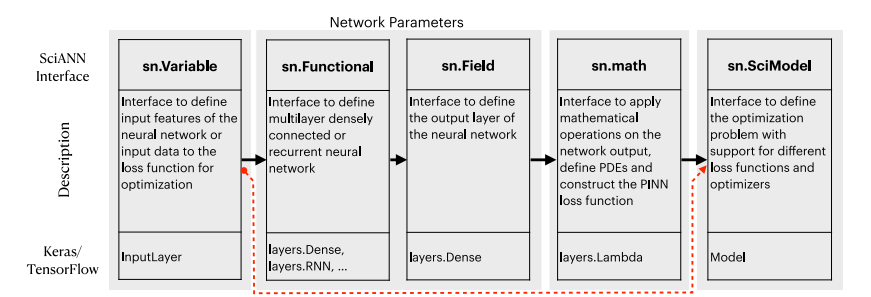
\includegraphics[width=1\textwidth]{img/img03.png}
    \caption{Elementos abstractos de \textit{SciANN} y su relación con capas de Keras y Tensowflow. Diagrama extraído de~\cite{Haghighat2021}.}
    \label{fig:img03}
\end{figure}

En el diagrama de la \autoref{fig:img03}, se muestra el flujo de creación de una PINN a través de cinco bloques. Los primeros tres bloques muestran cómo se mantiene una estructura secuencial entre la capa de variables de entrada, las capas de la función y la capa de salida. Entre las salidas podremos definir restricciones, relaciones y operaciones matemáticas, tal y como se muestra en el cuarto bloque. Son únicamente estas restricciones junto con los datos de entrada lo que debemos especificar para construir el modelo ---último bloque del procedimiento---, ya que los primeros tres bloques del diagrama quedan ``ligados'' a partir de las restricciones definidas en el cuarto bloque. 

Uno de los puntos clave de \textit{SciANN} es que al añadir capas de operaciones matemáticas a las salidas, estamos haciendo que estas operaciones sean la última capa de la red, esto es, las nuevas salidas. Así, la función de pérdida tomará esas operaciones en vez de las salidasde un elemento \textit{Functional}. 

\subsection{Espacio de datos}

Como mencionabamos en el apartado anterior, las entradas de una PINN en \textit{SciANN} definen las entradas de una función a aprender y se modelan mediante la clase \textit{Variable}. En esta sección, vamos a entender qué tipo de entradas requiere una PINN. 

A la hora de simular un fenómeno físico, debemos identificar los elementos que lo componen para estudiar cuál es el espacio que permite definir el fenómeno en su totalidad. Por ejemplo, los elementos a tener en cuenta cuando simulamos el calor transferido al ambiente en un disipador no serán los mismos que cuando queremos simular la distribución de cargas en una viga. 

De forma general, definimos el espacio de entrada de una PINN, denotado por $ S=(X,T) $, y en él las entradas como una distribución $S^*=(X^*,T^*)\subset S$ de puntos $(x^*,t^*)\in S^*$ distribuidos por el espacio a simular. Esto es, un mallado en el espacio cuya dimensionalidad, densidad, formato y otras cuestiones dependerán del fenómeno concreto a simular. En la~\autoref{fig:img3334} se muestran algunos ejemplos concretos de mallados válidos para PINNs. 

\begin{figure}[htbp]

    \begin{subfigure}{0.5\textwidth}
    \centering
    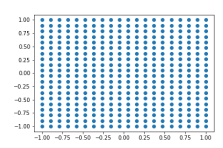
\includegraphics[width=0.7\linewidth]{img/img33.png} 
    \caption{Mallado uniforme centrado en $(0,0)$}
    \label{fig:img33}
    \end{subfigure}   
    \begin{subfigure}{0.5\textwidth}
    \centering
    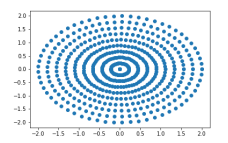
\includegraphics[width=0.7\linewidth]{img/img34.png}
    \caption{Mallado radial centrado en $(0,0)$}
    \label{fig:img34}
    \end{subfigure}

\caption{Ejemplos de mallado para PINNs}
\label{fig:img3334}
\end{figure}

\subsection{Entrenamiento}\label{sec:7.2.3}

Mientras que las PINNs originales proponían algoritmos de entrenamiento diferentes a la propagación hacia atrás, donde distintos conjuntos de datos (valores de entrada, funciones a modelar y sus restricciones) contribuían de forma independiente a la función de pérdida, la arquitectura de los modelos en \textit{SciANN} añade una capa \textit{Lambda} que describe esas restricciones simbólicas, lo que nos permite dar una equivalencia secuencial y unificada del problema y lo hace interpretable por Keras. 

A nivel formal, si queremos aprender una función $u$ cuyas entradas pertenecen a un espacio $S$, estas restricciones se pueden representar mediante relaciones de tipo 
\begin{equation}
    G(u) = F(u) 
\end{equation}

donde $G$ y $F$ son funcionales de tipo diferencial que actúan sobre $u$. Como el objetivo es representar estas relaciones como términos de la función de pérdida a minimizar, suelen reescribirse de forma
\begin{equation}
    H(u) = G(u) - F(u) = 0.
\end{equation}

Así, la función de pérdida asociada al problema de aprendizaje resulta:

\begin{equation}
    \mathcal{L}(\theta) = \sum (\sum_{S^*} \parallel u(x^*,t^*) - u_{\theta}(x^*,t^*)) \parallel + \sum_{S^*} \parallel H_i(u_{\theta}(x^*,t^*))\parallel.
\end{equation}
Por tanto, obtenemos una función de pérdida adecuada segun los requerimientos de las PINNs mientras que aprovehcamos las ventajas del entrenamiento de redes neuronales en Keras, entre ellas la paralelización y el mini-batch.




